\documentclass[11pt, fleqn]{article}

\usepackage{amsmath}
\usepackage{amssymb}
\usepackage{amsthm}
\usepackage{mathtools}
\usepackage{hyperref}
\usepackage{ulem}
\usepackage{enumitem}
\usepackage[left=0.75in, right=0.75in, bottom=0.75in]{geometry}
\usepackage{floatrow}
\usepackage{graphicx}
\usepackage[export]{adjustbox}

\usepackage{sectsty}
\sectionfont{\centering}

\usepackage[perpage]{footmisc}

\usepackage{fancyhdr}
\pagestyle{fancy}
\fancyhf{}
\lhead{190100044 \& 190100055}
\rhead{CS 215: Assignment 5}
\renewcommand{\footrulewidth}{1.0pt}
\cfoot{Page \thepage}

\setlength{\parindent}{0em}
\renewcommand{\arraystretch}{2}%

\title{Assignment 5: CS 215}
\author{
\begin{tabular}{|c|c|}
     \hline
     Devansh Jain & Harshit Varma \\
     \hline
     190100044 & 190100055 \\
     \hline
\end{tabular}
}
\date{\today}

\begin{document}

\maketitle

\renewcommand{\arraystretch}{1}

\section*{Question 1}
\addcontentsline{toc}{section}{Question 1}
\setcounter{equation}{0}
\setcounter{figure}{0}

\subsection*{Instructions for running the code}
\begin{enumerate}[itemsep=-1ex]
    \item Unzip, \texttt{cd} into \texttt{q1/code}, open and run \texttt{q1.m}
    \item The respective plots for MLE, MAP$_1$, and MAP$_2$ will be created and saved to \texttt{q1/results/}
\end{enumerate}

\subsection*{ML Estimate}
We know that ML estimate is the sample mean $=\boxed{\Bar{x}}$

\subsection*{MAP$_1$ Estimate:}
This was derived in class, $$\boxed{\frac{\sigma_0^2\Bar{x} + \sigma^2\mu_0/N}{\sigma_0^2 + \sigma^2/N}}$$

\subsection*{MAP$_2$ Estimate:}
Likelihood:
$$
    L(x|\mu) = C\cdot \exp{\sum_{i=1}^N\frac{(x_i-\mu)^2}{2\sigma^2}}
$$
Prior:
$$
\begin{aligned}
    P(\mu) &= \frac{1}{b-a} \hspace{1em} \text{If $a \le \mu \le b$}\\
    &= 0 \hspace{1em} \text{otherwise}
\end{aligned}
$$
Posterior is proportional to Likelihood$\times$Prior
$$
    \begin{aligned}
        F(\mu|x) &=  \frac{C}{b-a}\cdot \exp{\sum_{i=1}^N\frac{(\mu-x_i)^2}{2\sigma^2}}\\
        &= \frac{C'}{b-a}\cdot \exp{\frac{(\mu-\Bar{x})^2}{2\sigma^2/N}}
    \end{aligned}
$$
Thus, the maximum of the posterior is at $\Bar{x}$, which is same as the ML estimate.\\
But, if $\Bar{x} < a$, then we know from the prior that this is not possible, thus in this case, the MAP estimate will be $a$, similarly, if $\Bar{x} > b$, the MAP estimate will be $b$. Thus, the MAP$_2$ estimate can be written compactly as: $$\boxed{\min{(\max(\Bar{x}, a), b)}}$$

\subsection*{Boxplots:}

\begin{figure}[H]
    \centering
    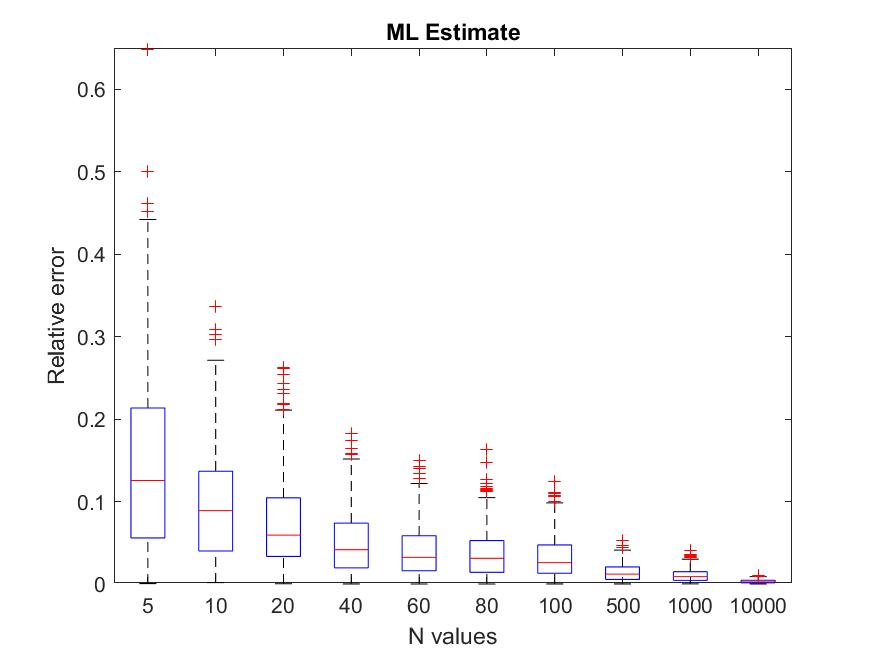
\includegraphics[scale=0.5]{q1/mle.jpg}
    \caption{ML Estimate relative error}
\end{figure}

\newpage

\begin{figure}[H]
    \centering
    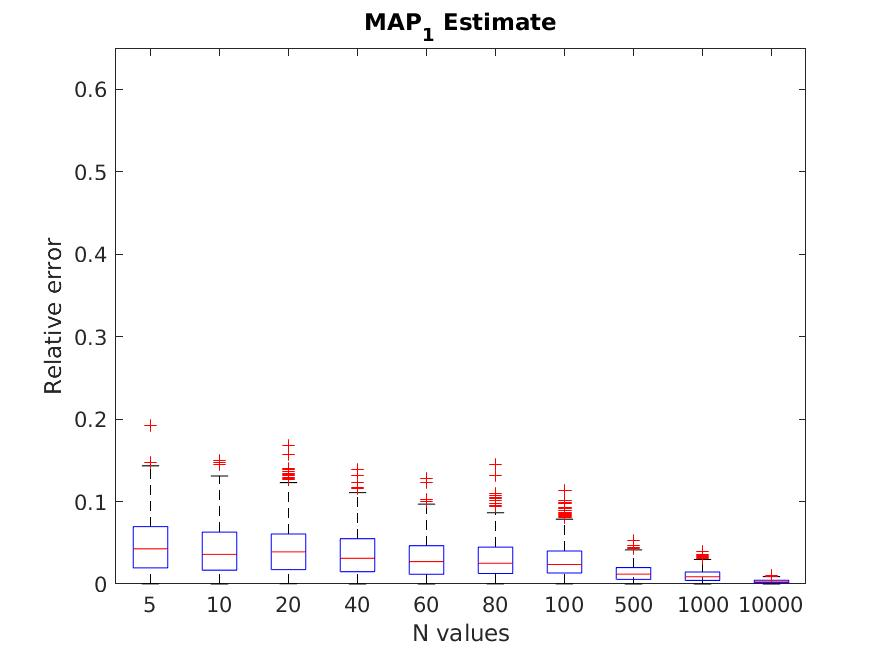
\includegraphics[scale=0.42]{q1/map1.jpg}
    \caption{MAP$_1$ Estimate relative error}
\end{figure}

\begin{figure}[H]
    \centering
    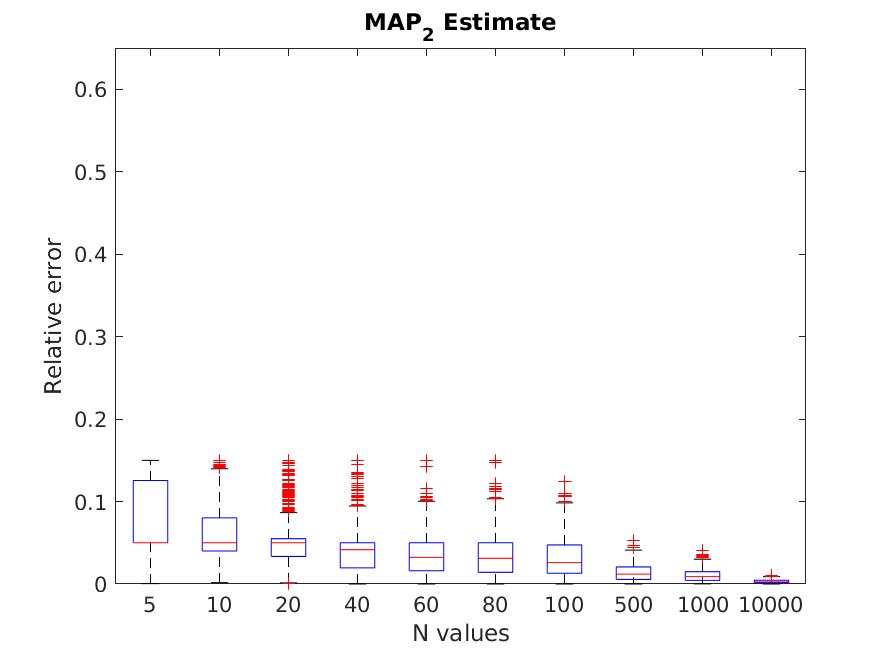
\includegraphics[scale=0.42]{q1/map2.jpg}
    \caption{MAP$_2$ Estimate relative error}
\end{figure}

\subsection*{Interpretation}
i.) The relative errors decrease to zero for all 3 estimates as $N$ increases, this is desirable.\\
ii.) When $N$ is small, MAP$_1$ estimate performs better than the others.\\
For large $N$, the three estimates perform approximately the same.\\
Due to the reasons stated above, we prefer the MAP$_1$ estimate over the other two.

\end{document}